\documentclass{report}
\usepackage{algorithmicx, algpseudocode, graphicx, imakeidx, hyperref}
\usepackage[a4paper, total={6in, 8in}]{geometry}

\makeindex

\begin{document}
\begin{titlepage}
  \begin{center}
    \textbf{\Large\\ SOEN 6441}
    \vspace{1cm}
    \textbf{\Huge\\ ADVANCED PROGRAMMING PRACTICES}
    \vspace{1cm}
    \Huge\\DELIVERABLE 1\\
    \vspace{1cm}
    \Large \textbf{TEAM E}\\
    \begin{large}
      \vspace{.5cm}
      Pouria Pirian (40207625)\\
      Sachin Prakash (40218678)\\
      Nishant	Saini (40195801)\\
      Chandra Sagar Reddy	Sangu (40234194)\\
      Omer Sayem (40226505)\\
      Kajal Sehrawat (40230025)\\
    \end{large}
    \begin{Large}
      
      \vspace{1 cm}
      Department of Computer Science and Software Engineering \\
      Gina Cody School of Engineering and Computer Science \\
      \textbf{Concordia University, Montreal}\\

      \vspace{1 cm}
      \today \\
    \end{Large}
  \end{center}

  \vfill
  \begin{center}
    
\includegraphics[width = 50ex]{resources/concordia_med.jpg}
  \end{center}
  
\end{titlepage}

\tableofcontents{}
\printindex{}

\chapter{Outline}
\section{Introduction}
  Coasters prevent condensation from dripping along the glass, which can damage the surface of tables. The project referred to as \textbf {CHEERS} deals with two circular coasters overlapping each other. The objective of \textbf {CHEERS} is to compute the diameter of the overlapping region such that 
  the real estate is half that of any of the coasters.

\section{Background}
  In this project, we determine the roots of an equation to calculate the angle made at the vertex of a coaster using the \textbf{Secant approximation method}. This method approximates the value of a function using a secant line passing through two points on a graph.
  $$ x_{n+1} = x_n - \frac{f(x_n) \cdot (x_n - x_{n-1})}{f(x_n) - f(x_{n-1})} $$

  \vspace*{20pt}
  \noindent The Sin/Cos value is approximated using the \textbf{Mclaurin Series} which is the sum of derivatives of a function.
  $$\sin(x) = \sum_{n=0}^{\infty} \frac{(-1)^n}{(2n+1)!}x^{2n+1}$$
  $$\cos(x) = \sum_{n=0}^{\infty} \frac{(-1)^n}{(2n)!}x^{2n}$$ 

\section{Scope}
  The length \textbf{l} of the overlapping coaster region can be computed by the equation
  $$l = 2R\left(1 - \cos\frac{\alpha}{2}\right)$$

  \indent R \textrightarrow \;radius of the coaster \\
  \indent $\alpha$ \textrightarrow \;angle created with the vertex at the centre point of the left coaster

  \vspace{20pt}
  The angle, $\alpha$ can be calculated using
  $$\alpha - \sin(\alpha) = \frac{\pi}{2}$$
  
  \vspace*{20pt}
  
  \begin{itemize}
    \item {The roots of the equation need to be determined to compute the value of $\alpha$. We use the Secant approximation method to arrive at a solution.}
    \item {The Mclaurin series has been used to approximate the Sin and Cos values and, subsequently, calculate l.}
  \end{itemize}

\section{Objectives}
\begin{itemize}
  \item To compute the value of $\Pi$.
  \item To compute the exponent of a number using recursion.
  \item To compute the factorial of a number using recursion.
  \item To approximate Sin and Cos using Mclaurin Series.
  \item To find the roots of an equation using Secant Approximation.
\end{itemize}

\section{Assumptions}
  The initial guess values for approximating the roots of an equation will be pre-determined.

\chapter{CRC Cards}
\begin{figure}[h!]
    \centering
    \begin{tabular}{@{}c@{}}
      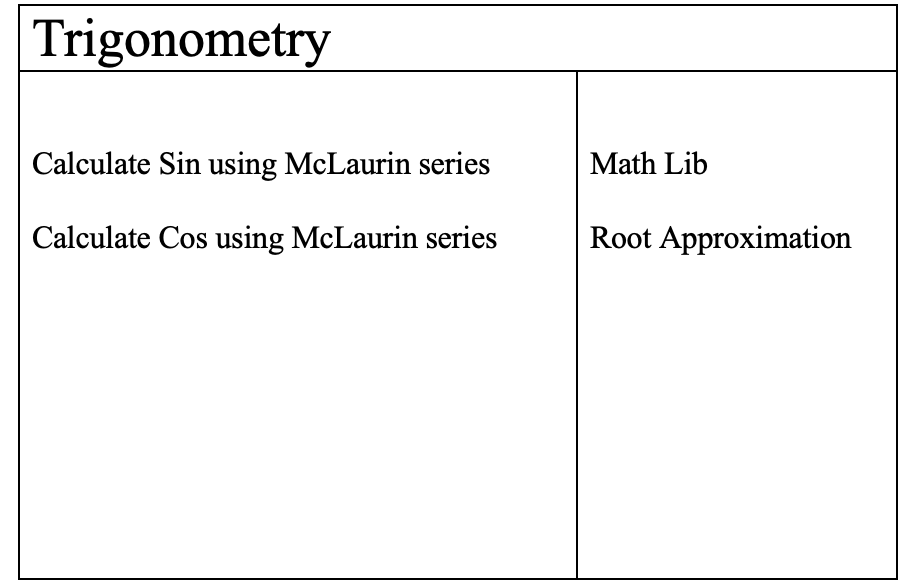
\includegraphics[width=.3\linewidth]{resources/Trigonometry.png} 
        \hspace*{30pt}
      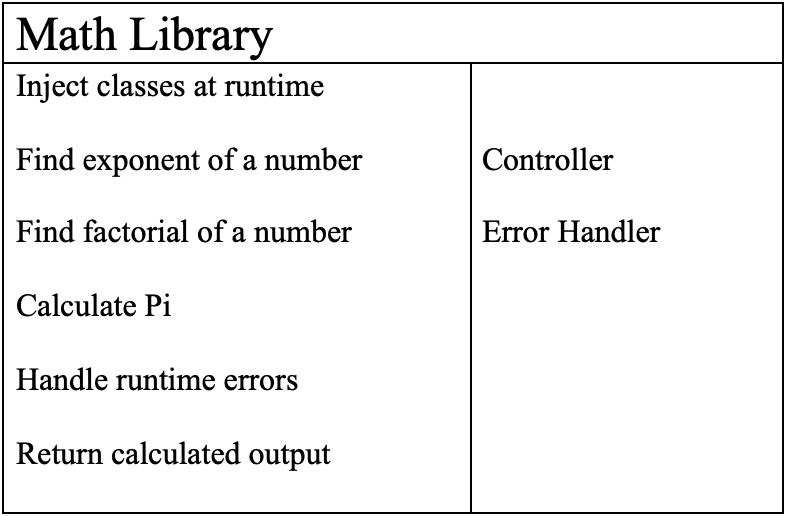
\includegraphics[width=.3\linewidth]{resources/MathLib.png}
    \end{tabular}
  
    \begin{tabular}{@{}c@{}}
        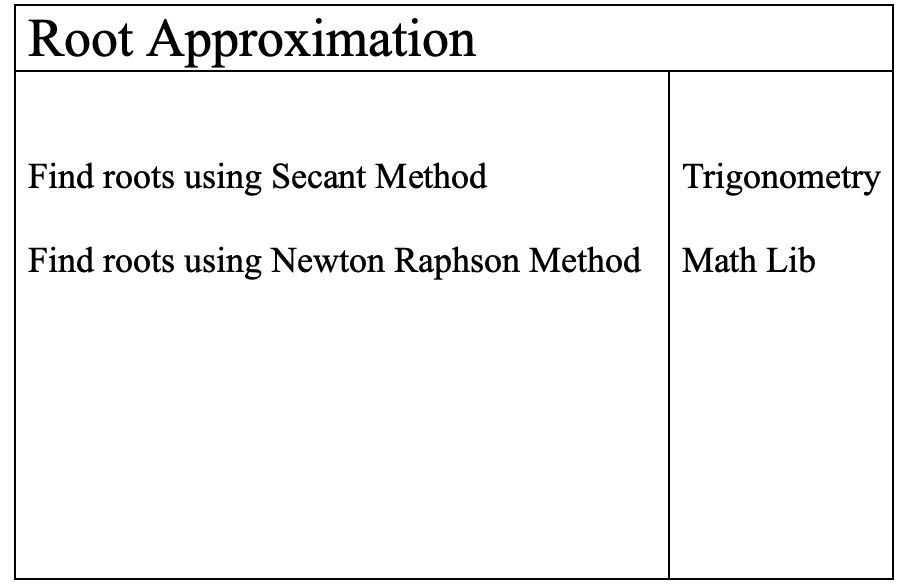
\includegraphics[width=.3\linewidth]{resources/RootApproximation.png} 
          \hspace*{30pt}
        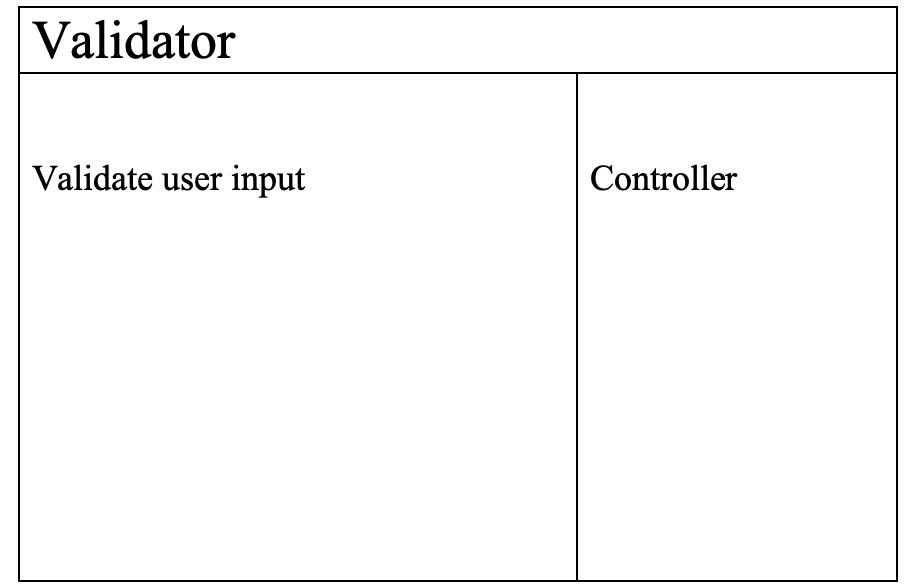
\includegraphics[width=.3\linewidth]{resources/Validator.png}
      \end{tabular}

      \begin{tabular}{@{}c@{}}
        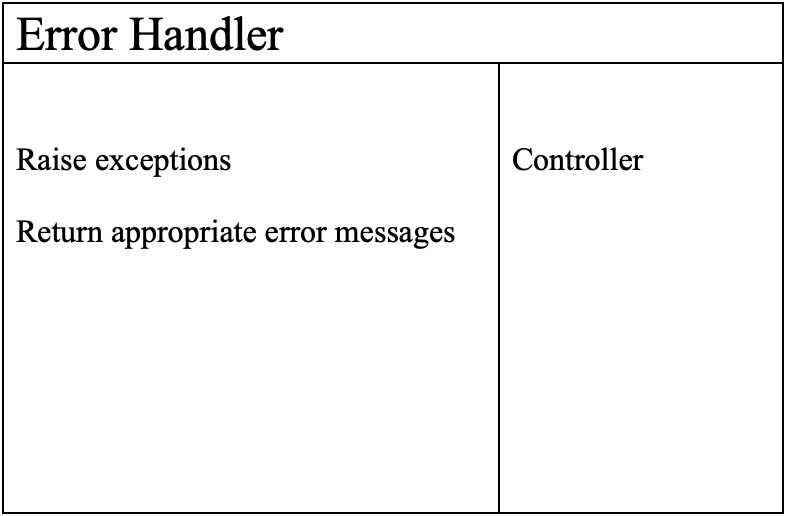
\includegraphics[width=.3\linewidth]{resources/ErrorHandler.png} 
          \hspace*{30pt}
        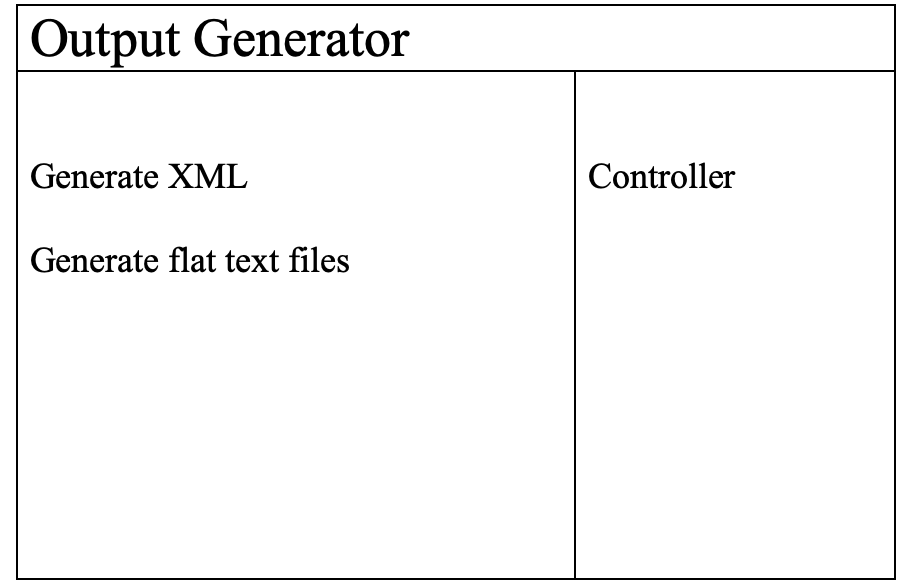
\includegraphics[width=.3\linewidth]{resources/OutputGenerator.png}
      \end{tabular}
      
      \begin{tabular}{@{}c@{}}
        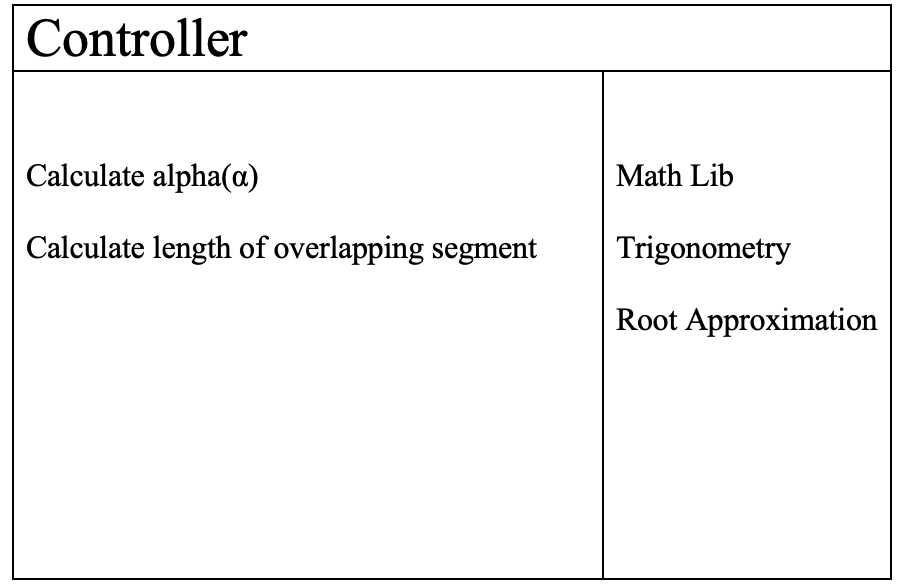
\includegraphics[width=.4\linewidth,height=90pt]{resources/Controller.png}
      \end{tabular}

      \vspace{\floatsep}
    \caption{CRC Cards for CHEERS}\label{fig:myfig}
\end{figure}

\chapter{Pseudocode}
\section{Sin using Mclaurin}
\begin{flushleft}
We arrive at a value for sin of a number using the Mclaurin series expansion \cite{doi:10.1137/1021091}.
\end{flushleft}
$$\sin(x) = \sum_{n=0}^{\infty} \frac{(-1)^n}{(2n+1)!}x^{2n+1}$$
% \break
\begin{algorithmic}[1]
    \Function{calculate\_sin}{$rad$}
        \State $total\_iterations \gets precision$
        \State $sin\_val \gets 0$
        \For{$i \gets 0, total\_iterations$}
            \State $term \gets (-1)^i \cdot rad^{2i + 1} / (2i + 1)!$
            \State $sin\_val \gets sin\_val + term$
        \EndFor
        \State \Return $sin\_val$
    \EndFunction
\end{algorithmic}
\begin{flushleft}
There are various methods of calculating sin of a number using various infinite series like Taylor series, Maclauren series, power series and Euler's formula.
While each of the methods have advantages and disadvantages of their own, Mclaurin Series has some distinct advantages over other methods.They are as follows :
\end{flushleft}
\begin{itemize}
  \item \textbf{Simplicity} : Maclaurin Series simple to use, as it only uses relatively simple mathematical functions. Due to the same reason it is easy to implement a computer program of it.
  \item \textbf{Convergence} : The Maclaurin series converges for all values of x, which means that it can be used to calculate the sine function accurately for any angle.
  \item  \textbf{Accuracy} : The accuracy of Maclaurin series increases with every new term that is added.So, with every iteration it rapidly converges to true value of sin.
  \item \textbf{Versatility}: The Maclaurin series can be easily extended to calculate other trigonometric functions, such as cosine and tangent, by simply changing the coefficients of the terms in the series.
\end{itemize}
\section{Secant Approximation}
\begin{flushleft}
The roots of an equation can be derived using the secant approximation method \cite{Wikipedia:SecantMethod}.
\end{flushleft}
$$ x_{n+1} = x_n - \frac{f(x_n) \cdot (x_n - x_{n-1})}{f(x_n) - f(x_{n-1})} $$
% \break
\begin{algorithmic}[1]
\Function{secant\_approximation}{func, $x_0$, $x_1$, $e$}
    \State $x_2 \gets 0$
    \State $step \gets 1$
    \While{True}
        \If{func($x_0$) == func($x_1$)}
            \State \textbf{break}
        \EndIf
        \State $x_2 \gets x_0 - (x_1 - x_0) * func(x_0) / (func(x_1) - func(x_0))$
        \State $x_0 \gets x_1$
        \State $x_1 \gets x_2$
        \State $step \gets step + 1$
        \If{$step > num\_terms$}
            \State \textbf{print}("Not convergent")
            \State \textbf{break}
        \EndIf
        \If{func($x_2$) - func($x_1$) $>$ e}
            \State \textbf{break}
        \EndIf
    \EndWhile
    \State \textbf{return} $x_2$
\EndFunction
\end{algorithmic}
\begin{flushleft}
  The secant method is similar to the Newton-Raphson method, but it uses an approximation of the derivative instead of the actual derivative. Secant method has various advantages over other methods like bisection method and Newton-Raphson method. They are as follows:
  \begin{itemize}
    \item \textbf{No derivative required} : One of the main advantage of secant method is that we do not need to calculate the derivative of the function whose roots we are trying to calculate. So, writing a program is lot easire that that of Newton-Raphson method, which requires derivative of the function.
    \item \textbf{Convergence rate} : The secant method has a convergence rate that is faster than the bisection method but slower than the Newton-Raphson method. However, it is less likely to diverge than the Newton-Raphson method.
    \item \textbf{Applicability to nonlinear functions}: The secant method is applicable to nonlinear functions, whereas the bisection method is applicable only to continuous functions that change sign over an interval.
    \item \textbf{Multiple roots} : Unlike bisection method, secant method can detect multiple roots in a given interval.
  \end{itemize}
\end{flushleft}

\section{Pi Calculation}
\begin{flushleft}
  The value of pi is calculated using Leibniz formula.
\end{flushleft}
$${\frac {\pi }{4}}=\sum _{k=0}^{\infty }{\frac {(-1)^{k}}{2k+1}}$$
% \break
\begin{algorithmic}[1]
    \Function{CalculatePi}{}
        \State $val \gets 0.0$
        \State $total\_terms \gets 100$
        \For{$i=1$ to $2*total\_terms$}
            \State $sign \gets -(i\%4-2)$
            \State $val \gets val + \frac{sign}{i}$
        \EndFor
        \State \Return $4 * val$
    \EndFunction
\end{algorithmic}
\begin{flushleft}
  Leibniz formula is a special case of $arctan(x)$ series, that is as follows.
  $$\arctan x=x-{\frac {x^{3}}{3}}+{\frac {x^{5}}{5}}-{\frac {x^{7}}{7}}+\cdots$$
  When x is equal to 1, we get $\arctan(1) = {\frac{1}{4}}\pi.$
  The advantages of Leibniz formula is as follows:
  \begin{itemize}
    \item \textbf{Simple implementation} : It is a simple formula that can be easily programmed, as it requires only basic mathematical operations like power and division.
    \item \textbf{Accuracy} : The Leibniz formula gives an accurate approximation of $\pi$, with each additional term of the series increasing the accuracy of the approximation.The formula can be used to calculate $\pi$ to any desired level of precision, depending on how many terms of the series are used.
  \end{itemize}
\end{flushleft}
\section{Exponent}
\begin{flushleft}
The exponent of a number can be obtained using the following algorithm.
\end{flushleft}
% \break
\begin{algorithmic}[1]
\Function{exp}{$number$, $power$}
    \If{$power = 0$}
        \State \Return $1$
    \EndIf
    \State $temp \gets$ \Call{exp}{$number$, $\lfloor power/2 \rfloor$}
    \If{$power$ is even}
        \State \Return $temp * temp$
    \Else
        \State \Return $temp * temp * number$
    \EndIf
\EndFunction
\end{algorithmic}
\vspace{2cm}
\begin{flushleft}
  The above algorithm is preferred over naive approach as it require less number of recursive function calls.
  The naive approach can quickly become impractical or even impossible for very large exponents, as the number of multiplications required grows exponentially with the size of the exponent. The exponentiation by squaring approach, on the other hand, uses recursive halving of the exponent to reduce the number of multiplications required, making it more practical for large exponents.
\end{flushleft}
\section{Factorial}
\begin{flushleft}
This is the algorithm used to obtain the factorial of a number.
\end{flushleft}
% \break
\begin{algorithmic}[1]
\Function{factorial}{$num$}
  \If{$num < 0$}
    \State \textbf{raise} Exception(``Factorial can't be calculated for negative numbers'')
  \EndIf
  \State $result \gets 1$
  \For{$i \gets 1$ \textbf{to} $num$}
    \State $result \gets result \times i$
  \EndFor
  \State \textbf{return} $result$
\EndFunction
\end{algorithmic}

\bibliographystyle{unsrt}
\bibliography{citation}
\printindex
\end{document}